\documentclass[10pt]{article}\usepackage[]{graphicx}\usepackage[]{color}
%% maxwidth is the original width if it is less than linewidth
%% otherwise use linewidth (to make sure the graphics do not exceed the margin)
\makeatletter
\def\maxwidth{ %
  \ifdim\Gin@nat@width>\linewidth
    \linewidth
  \else
    \Gin@nat@width
  \fi
}
\makeatother

\definecolor{fgcolor}{rgb}{0.345, 0.345, 0.345}
\newcommand{\hlnum}[1]{\textcolor[rgb]{0.686,0.059,0.569}{#1}}%
\newcommand{\hlstr}[1]{\textcolor[rgb]{0.192,0.494,0.8}{#1}}%
\newcommand{\hlcom}[1]{\textcolor[rgb]{0.678,0.584,0.686}{\textit{#1}}}%
\newcommand{\hlopt}[1]{\textcolor[rgb]{0,0,0}{#1}}%
\newcommand{\hlstd}[1]{\textcolor[rgb]{0.345,0.345,0.345}{#1}}%
\newcommand{\hlkwa}[1]{\textcolor[rgb]{0.161,0.373,0.58}{\textbf{#1}}}%
\newcommand{\hlkwb}[1]{\textcolor[rgb]{0.69,0.353,0.396}{#1}}%
\newcommand{\hlkwc}[1]{\textcolor[rgb]{0.333,0.667,0.333}{#1}}%
\newcommand{\hlkwd}[1]{\textcolor[rgb]{0.737,0.353,0.396}{\textbf{#1}}}%
\let\hlipl\hlkwb

\usepackage{framed}
\makeatletter
\newenvironment{kframe}{%
 \def\at@end@of@kframe{}%
 \ifinner\ifhmode%
  \def\at@end@of@kframe{\end{minipage}}%
  \begin{minipage}{\columnwidth}%
 \fi\fi%
 \def\FrameCommand##1{\hskip\@totalleftmargin \hskip-\fboxsep
 \colorbox{shadecolor}{##1}\hskip-\fboxsep
     % There is no \\@totalrightmargin, so:
     \hskip-\linewidth \hskip-\@totalleftmargin \hskip\columnwidth}%
 \MakeFramed {\advance\hsize-\width
   \@totalleftmargin\z@ \linewidth\hsize
   \@setminipage}}%
 {\par\unskip\endMakeFramed%
 \at@end@of@kframe}
\makeatother

\definecolor{shadecolor}{rgb}{.97, .97, .97}
\definecolor{messagecolor}{rgb}{0, 0, 0}
\definecolor{warningcolor}{rgb}{1, 0, 1}
\definecolor{errorcolor}{rgb}{1, 0, 0}
\newenvironment{knitrout}{}{} % an empty environment to be redefined in TeX

\usepackage{alltt}

\usepackage{amsmath,amssymb,amsthm}
\usepackage{fancyhdr,url,hyperref}
\usepackage{graphicx,xspace}
\usepackage{subfigure}
\usepackage{tikz}
\usetikzlibrary{arrows,decorations.pathmorphing,backgrounds,positioning,fit,through}

\oddsidemargin 0in  %0.5in
\topmargin     0in
\leftmargin    0in
\rightmargin   0in
\textheight    9in
\textwidth     6in %6in
%\headheight    0in
%\headsep       0in
%\footskip      0.5in

\newtheorem{thm}{Theorem}
\newtheorem{cor}[thm]{Corollary}
\newtheorem{obs}{Observation}
\newtheorem{lemma}{Lemma}
\newtheorem{claim}{Claim}
\newtheorem{definition}{Definition}
\newtheorem{question}{Question}
\newtheorem{answer}{Answer}
\newtheorem{problem}{Problem}
\newtheorem{solution}{Solution}
\newtheorem{conjecture}{Conjecture}

\pagestyle{fancy}

\lhead{\textsc{Prof. McNamara}}
\chead{\textsc{SDS/MTH 220: Lecture notes}}
\lfoot{}
\cfoot{}
%\cfoot{\thepage}
\rfoot{}
\renewcommand{\headrulewidth}{0.2pt}
\renewcommand{\footrulewidth}{0.0pt}

\newcommand{\ans}{\vspace{0.25in}}
\newcommand{\R}{{\sf R}\xspace}
\newcommand{\cmd}[1]{\texttt{#1}}

\rhead{\textsc{October 6, 2017}}
\IfFileExists{upquote.sty}{\usepackage{upquote}}{}
\begin{document}

\paragraph{Agenda}
\begin{enumerate}
  \itemsep0em
  \item Project groups due today
  \item Randomization test recap
  \item Hypothesis testing
\end{enumerate}

% \paragraph{Exam 1 Recap}
% The average was 84.6. I am implementing a bootstrap incentive. The threshold for this exam is 80. If you scored below the threshold, your score on \emph{this exam} will be retroactively raised to 80 if you score above the threshold on either of the remaining exams.  


\paragraph{Randomization test recap}

In the last class, we designed a simulation to help us answer the question of whether exposure to mites was associated, \emph{to a statistically significant} degree, with a decrease in wilt disease after exposure to Verticillium, a fungus that causes wilt disease. 

Most of us used the `no-wilt-mites' cell in the table as our test statistic. But there are other statistics we might have been interested in. Particularly, we might be interested in the difference in the proportion of plants that wilted between the mites and the no mites groups. To answer this question, we might
\begin{enumerate}
\item Count out 19 black cards (no wilt) and 28 red cards (wilt)
\item Shuffle
\item Deal into two piles: 26 (mites) and 21 (no mites)
\item Calculate the proportions of wilt (red cards) for each pile, then finally, the difference in proportions. Record your simulation and do steps 1-4 a bunch more times!
\end{enumerate}

\paragraph{Questions}
\begin{enumerate}
  \itemsep0.75in
  \item What is the \emph{null hypothesis} for this simulation?
  \item What is the \emph{test statistic}?
  \item Where does the test statistic lie in the \emph{null distribution}?
  \item Does this evidence cause you to \emph{reject} or \emph{fail to reject} the null hypothesis?
  \item Write \emph{one} sentence summarizing what you've learned about mites and wilt disease.  
  \vspace{0.5in}
\end{enumerate}

\begin{knitrout}\footnotesize
\definecolor{shadecolor}{rgb}{0.969, 0.969, 0.969}\color{fgcolor}\begin{kframe}
\begin{alltt}
\hlkwd{require}\hlstd{(mosaic)}
\hlkwd{tally}\hlstd{(}\hlopt{~} \hlstd{outcome} \hlopt{+} \hlstd{treatment,} \hlkwc{data} \hlstd{= Mites)}
\end{alltt}
\begin{verbatim}
##          treatment
## outcome   mites no mites
##   no wilt    15        4
##   wilt       11       17
\end{verbatim}
\begin{alltt}
\hlkwd{tally}\hlstd{(outcome} \hlopt{~} \hlstd{treatment,} \hlkwc{data} \hlstd{= Mites,} \hlkwc{format} \hlstd{=} \hlstr{"proportion"}\hlstd{)}
\end{alltt}
\begin{verbatim}
##          treatment
## outcome       mites  no mites
##   no wilt 0.5769231 0.1904762
##   wilt    0.4230769 0.8095238
\end{verbatim}
\end{kframe}
\end{knitrout}

\begin{knitrout}\footnotesize
\definecolor{shadecolor}{rgb}{0.969, 0.969, 0.969}\color{fgcolor}\begin{kframe}
\begin{alltt}
\hlstd{tbl} \hlkwb{<-} \hlkwd{tally}\hlstd{(outcome} \hlopt{~} \hlstd{treatment,} \hlkwc{data} \hlstd{= Mites,} \hlkwc{format} \hlstd{=} \hlstr{"proportion"}\hlstd{)}
\hlstd{diff_prop} \hlkwb{<-} \hlstd{tbl[}\hlnum{2}\hlstd{,}\hlnum{2}\hlstd{]} \hlopt{-} \hlstd{tbl[}\hlnum{2}\hlstd{,}\hlnum{1}\hlstd{]}
\hlstd{diff_prop}
\end{alltt}
\begin{verbatim}
## [1] 0.3864469
\end{verbatim}
\end{kframe}
\end{knitrout}

\begin{knitrout}\footnotesize
\definecolor{shadecolor}{rgb}{0.969, 0.969, 0.969}\color{fgcolor}\begin{kframe}
\begin{alltt}
\hlstd{null_dist} \hlkwb{<-} \hlkwd{do}\hlstd{(}\hlnum{5000}\hlstd{)} \hlopt{*} \hlkwd{tally}\hlstd{(outcome} \hlopt{~} \hlkwd{shuffle}\hlstd{(treatment),} \hlkwc{data} \hlstd{= Mites)}
\hlstd{null_dist} \hlkwb{<-} \hlstd{null_dist} \hlopt
\hlkwd{mutate}\hlstd{(}\hlkwc{prop_wilt_nomites} \hlstd{= wilt.no.mites}\hlopt{/}\hlstd{(wilt.no.mites}\hlopt{+}\hlstd{no.wilt.no.mites))} \hlopt
\hlkwd{mutate}\hlstd{(}\hlkwc{prop_wilt_mites} \hlstd{= wilt.mites}\hlopt{/}\hlstd{(wilt.mites}\hlopt{+}\hlstd{no.wilt.mites))} \hlopt
\hlkwd{mutate}\hlstd{(}\hlkwc{diff_prop} \hlstd{= prop_wilt_nomites} \hlopt{-} \hlstd{prop_wilt_mites)}
\hlkwd{ggplot}\hlstd{(}\hlkwc{data} \hlstd{= null_dist,} \hlkwd{aes}\hlstd{(diff_prop))} \hlopt{+}
\hlkwd{geom_histogram}\hlstd{(}\hlkwc{bins} \hlstd{=} \hlnum{10}\hlstd{)}
\end{alltt}
\end{kframe}
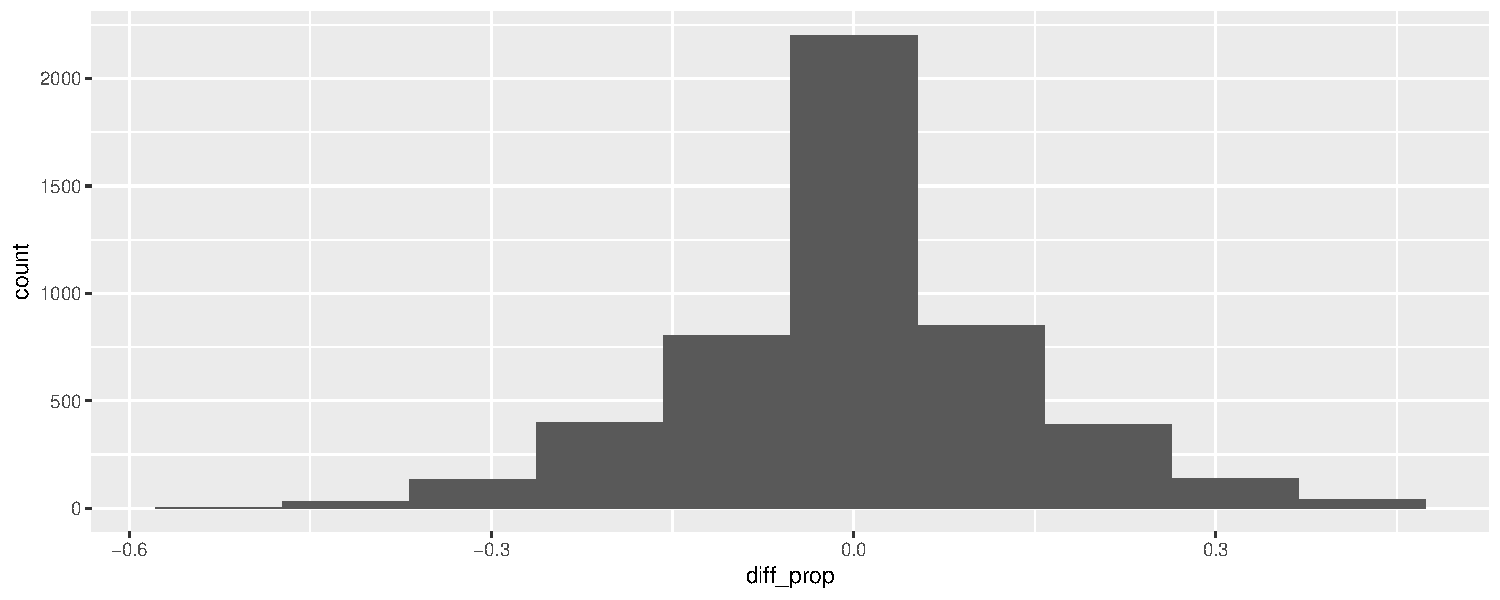
\includegraphics[width=\maxwidth]{figure/unnamed-chunk-3-1} 

\end{knitrout}

\begin{knitrout}\footnotesize
\definecolor{shadecolor}{rgb}{0.969, 0.969, 0.969}\color{fgcolor}\begin{kframe}
\begin{alltt}
\hlnum{2} \hlopt{*} \hlkwd{pdata}\hlstd{(}\hlopt{~}\hlstd{diff_prop,} \hlkwc{q}\hlstd{=}\hlnum{.3864}\hlstd{,} \hlkwc{data}\hlstd{=null_dist,} \hlkwc{lower.tail}\hlstd{=}\hlnum{FALSE}\hlstd{)}
\end{alltt}
\begin{verbatim}
## [1] 0.0156
\end{verbatim}
\end{kframe}
\end{knitrout}



\clearpage
\paragraph{What's Wrong?}

% MMC, 7e, 6.50, 6.51, page 378
Here are several situations where there is an incorrect application of the ideas presented in this section. Write a short paragraph explaining what is wrong in each situation and why it is wrong. 

\begin{enumerate}
  \itemsep0.5in
  \item A researcher tests the following null hypothesis: $H_0 : \bar{x} = 23$
  \item A study with $\bar{x} = 45$ reports statistical significance for $H_a : \mu > 50$. 
  \item A researcher tests the hypothesis $H_0 : \mu = 350$ and concludes that the population mean is equal to 350. 
  \item A test preparation company wants to test that the average score of their students on the ACT is better than the national average score of 21.1. They state their null hypothesis to be $H_0 : \mu > 21.2$. 
  \item A study summary says that the results are statistically significant and the p-value is 0.98. 
\end{enumerate}
% 
% \newpage
% 
% \subsection*{Instructor's Notes}
% 
% 
% \paragraph{Tests of Significance}
% 
% \begin{itemize}
%   \item Important concepts in hypothesis testing:
%   \begin{itemize}
%     \item $H_0$: null hypothesis - the state of the world that you assume is true. Typically, this is a world of ``no effect," in which probability distributions are easy to calculate or simulate. $H_0$ is a specific mathematical statement about a population parameter.
%     \item $H_A$: alternative hypothesis - a state of the world different from the null. Typically, this is a world in which the effect you are testing is real
%     \item test statistic: the estimate that you are testing. Typically, this is a something that you have computed from data and are trying to understand in the context of the null distribution
%     \item null distribution: the sampling distribution of the test statistic under the null hypothesis.
%     \item $p$-value: probability of observing something as strange or stranger as what you observed, \emph{under the assumption that the null hypothesis is true}
%     \item $\alpha$-level: a threshold beyond which you begin to doubt the null hypothesis. This is a line in the sand that you draw to purposefully gauge your dubiousness.
%   \end{itemize}
%   \item Two possible outcomes: 
%   \begin{itemize}
%     \item Reject $H_0$ at $\alpha$-significance level: observations are so unlikely under the null hypothesis, that it is likely false
%     \item Fail to reject $H_0$ at $\alpha$-significance level: observations are reasonably likely under null hypothesis, so can't rule out possibility that it is true
%   \end{itemize}
%   \item Important: we never confirm the null hypothesis -- we only fail to reject!
%   \item Always report $p$-values and a confidence interval
%   \item One-sided vs. two-sided tests: one-sided test are almost never used in practice
% \end{itemize}
% 
% \paragraph{Testing Outcomes}
% 
% For a defendant on trial:
% \begin{itemize}
%   \item $H_0$: innocent until proven guilty
%   \item Type I error: $\Pr(\text{reject} | H_0)$ - convicting an innocent person
%   \item Type II error: $\Pr(\text{fail to reject} | H_0^c) = 1- Power$ - letting a guilty person go free
% \end{itemize}
% 
% \begin{table}[b]
% \centering
% \begin{tabular}{|c|c|c|}
%   \hline
%   Decision \textbackslash Truth & $H_0$ is true & $H_0$ is false \\
%   \hline
%   Reject & \hspace{1.5in} & \hspace{1.5in} \\
%   \hline
%   Fail to Reject &  & \\
%   \hline
% \end{tabular}
% \end{table}


\end{document}
